\section{Durchführung}
\label{sec:Durchführung}

Die erste Messaufgabe besteht aus der direkten Messung der Leerlaufspannung einer
Monozelle. Dies geschieht über ein hochohmiges Voltmeter. Der Eingangswiderstand
$R_\text{V}$ und die abgelesene Leerlaufspannung wird notiert.
Danach wird die Schaltung mit dem Schaltbild, welches in Abbildung \ref{fig:schaltbild}
zu sehen ist, aufgebaut.

\begin{figure}
  \centering
  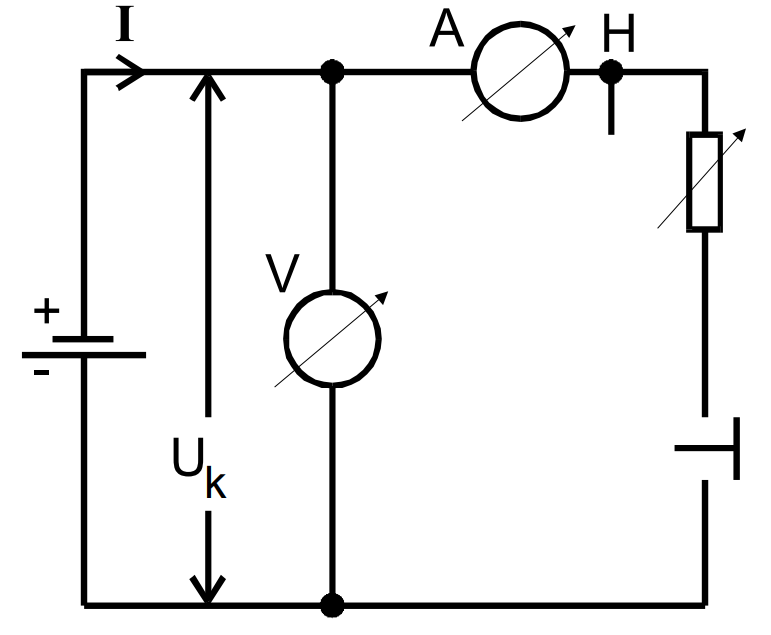
\includegraphics[width=150pt]{data/schaltbild1.png}
  \caption{Schaltbild zur Reihenschaltung einer realen Spannungsquelle mit einer Last und Messgeräten \cite{Versuchsanleitung}}
  \label{fig:schaltbild1}
\end{figure}

Der Lastwiderstand $R_\text{a}$ ist dabei in einem Bereich von $0$ bis
$\SI{50}{\ohm}$ regelbar. Über die Variation des Lastwiderstand wird die Stromstärke
, welche durch das vor den Lastwiderstand geschaltete Amperemeter gemessen wird,
verändert. Dadurch lässt sich die Klemmenspannung $U_\text{K}$ in Abhängkeit der
Stromstärke $I$ aufnehmen.

Nun wird hinter den regelbaren Widerstand eine Gegenspannung geschaltet, welche
ungefähr $\SI{2}{\volt}$ über der bereits näherungsweise gemessenen Leerlaufspannung
liegt.

\begin{figure}
  \centering
  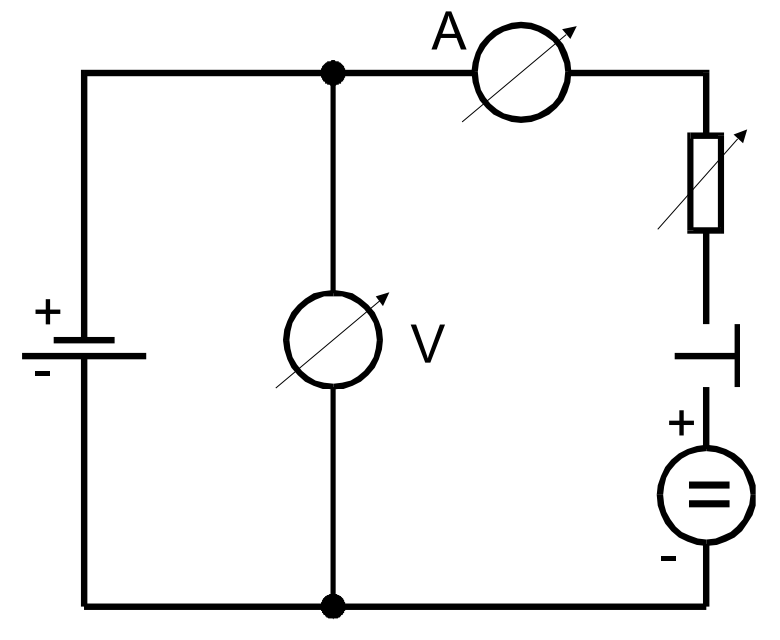
\includegraphics[width=150pt]{data/schaltbild2.png}
  \caption{Schaltbild zur gleichen Schaltung, jedoch mit einer Gegenspannung \cite{Versuchsanleitung}}
  \label{fig:schaltbild2}
\end{figure}
